\documentclass[11pt,a4paper]{article}

% Packages
\usepackage[utf8]{inputenc}
\usepackage[margin=1in]{geometry}
\usepackage{graphicx}
\usepackage{float}
\usepackage{amsmath}
\usepackage{hyperref}
\usepackage{booktabs}
\usepackage{enumitem}
\usepackage{caption}
\usepackage{natbib}
\usepackage{graphicx}

% Title information
\title{\textbf{Retail Customer Analysis}}
\author{Millan Das \and Arthur de Leusse \and Alexis Vannson}
\date{\today}

\begin{document}

\maketitle

\section*{Executive Summary}

We looked into retail customer data to support supermarkets with predictions of response rates for their marketing campaigns and their churn rate to help them allocate their resources in the most effective way. We worked on a dataset of 2,240 customer records with three approaches: customer segmentation through clustering, campaign response prediction, and churn prediction.

\textbf{Key findings:}
\begin{itemize}
    \item \textbf{Customer Segmentation:} k-means and DBSCAN revealed that the customer base was very homogeneous and could not be properly segmented using the current data (silhouette score 0.15 or non-representative cluster sizes).
    \item \textbf{Campaign Response Prediction:} Logistic regression achieved the strongest performance (ROC-AUC: 0.90, precision: 70\%), which could reduce costs through targeted marketing.
    \item \textbf{Churn Prediction:} XGBoost demonstrated moderate but actionable performance (accuracy: 60\%, ROC-AUC: 0.64), identifying the top 20\% highest-risk customers for proactive retention interventions.
\end{itemize}

These models provide a data-driven approach to marketing support that could improve ROI significantly with improved targeting campaigns and churn reduction, which is essential to the customer lifetime value.

\section{Introduction}

It has been observed that an increase in customer retention by only 5\% can create non-linear return and boost profits by 25\% to 95\% \citep{reichheld1990}. This finding emphasizes the strategic value of accurately understanding customer behavior and needs. With the recent increase of data quantity and computational power, the ability for companies to personalize their advertisement and retail strategies rose. This project's goal is to assess the effectiveness of machine learning techniques in generating deep consumer insights. The data we used is retail oriented and comes from Kaggle \citep{imakash3011}. The link of the Github repository where we did our analysis is given in the Bibliography.

\section{Models and Evaluation Measures}

\subsection{Clustering}

The K-means algorithm due to its simplicity and ease of interpretation. Using the elbow rule we concluded that the optimal $k$ was 4. We used silhouette score in order to estimate the performance of the clustering algorithm. Since its value was of 0.15 which is significantly lower than the threshold value of 0.5 that indicates acceptable clustering we decided to try the DBSCAN algorithm. We found that the best epsilon value was 7.5 using the elbow method for DBSCAN. Its result was unconvincing with one cluster found and 63 points labelled as noise. We thus concluded that the clustering for this data was meaningless hence that the clients of this retail store appear to form a relatively homogeneous population.


\vspace*{0.5cm}
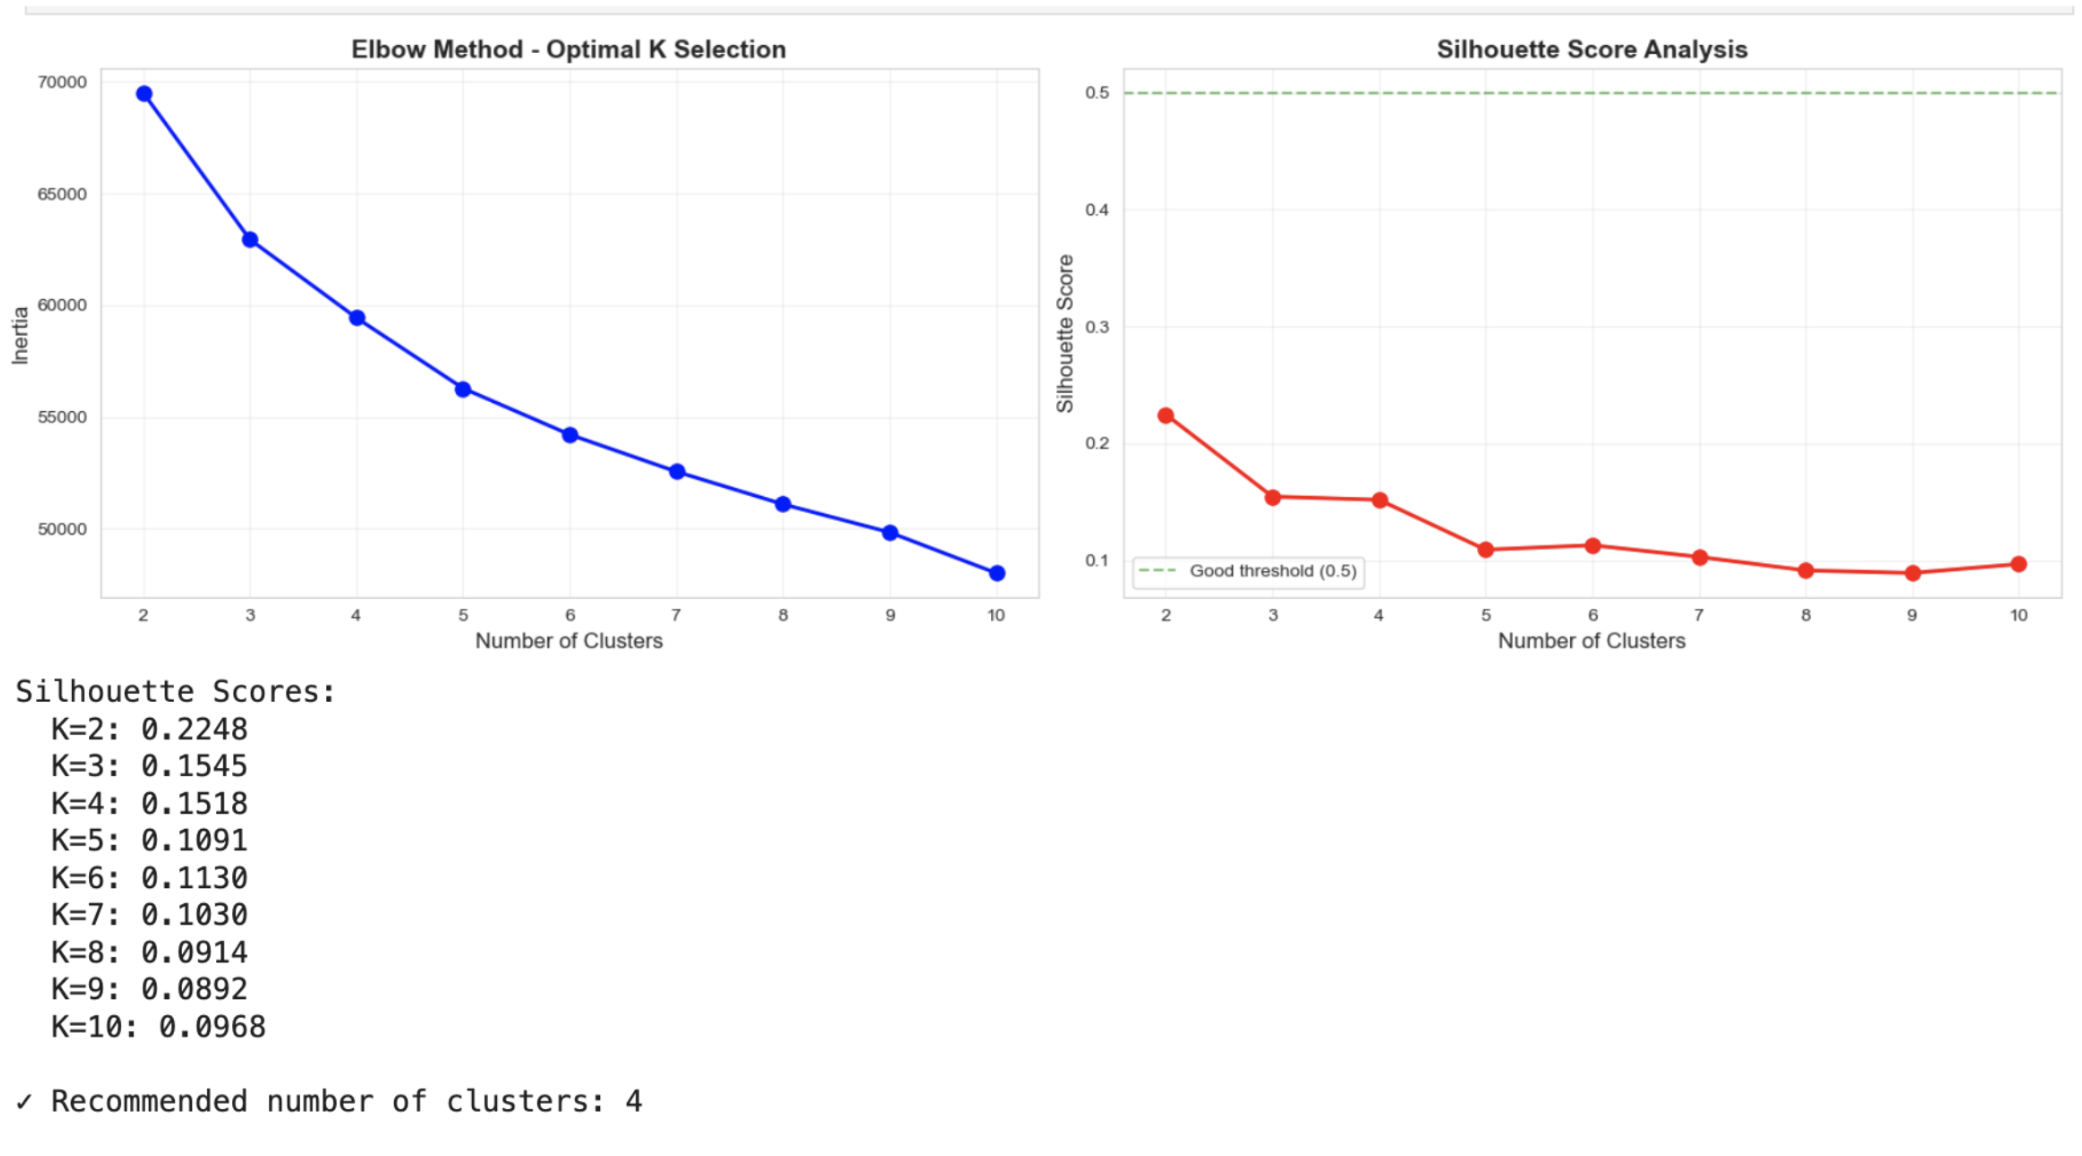
\includegraphics[width=0.95\textwidth]{silhouette.png}

\vspace*{0.5cm}
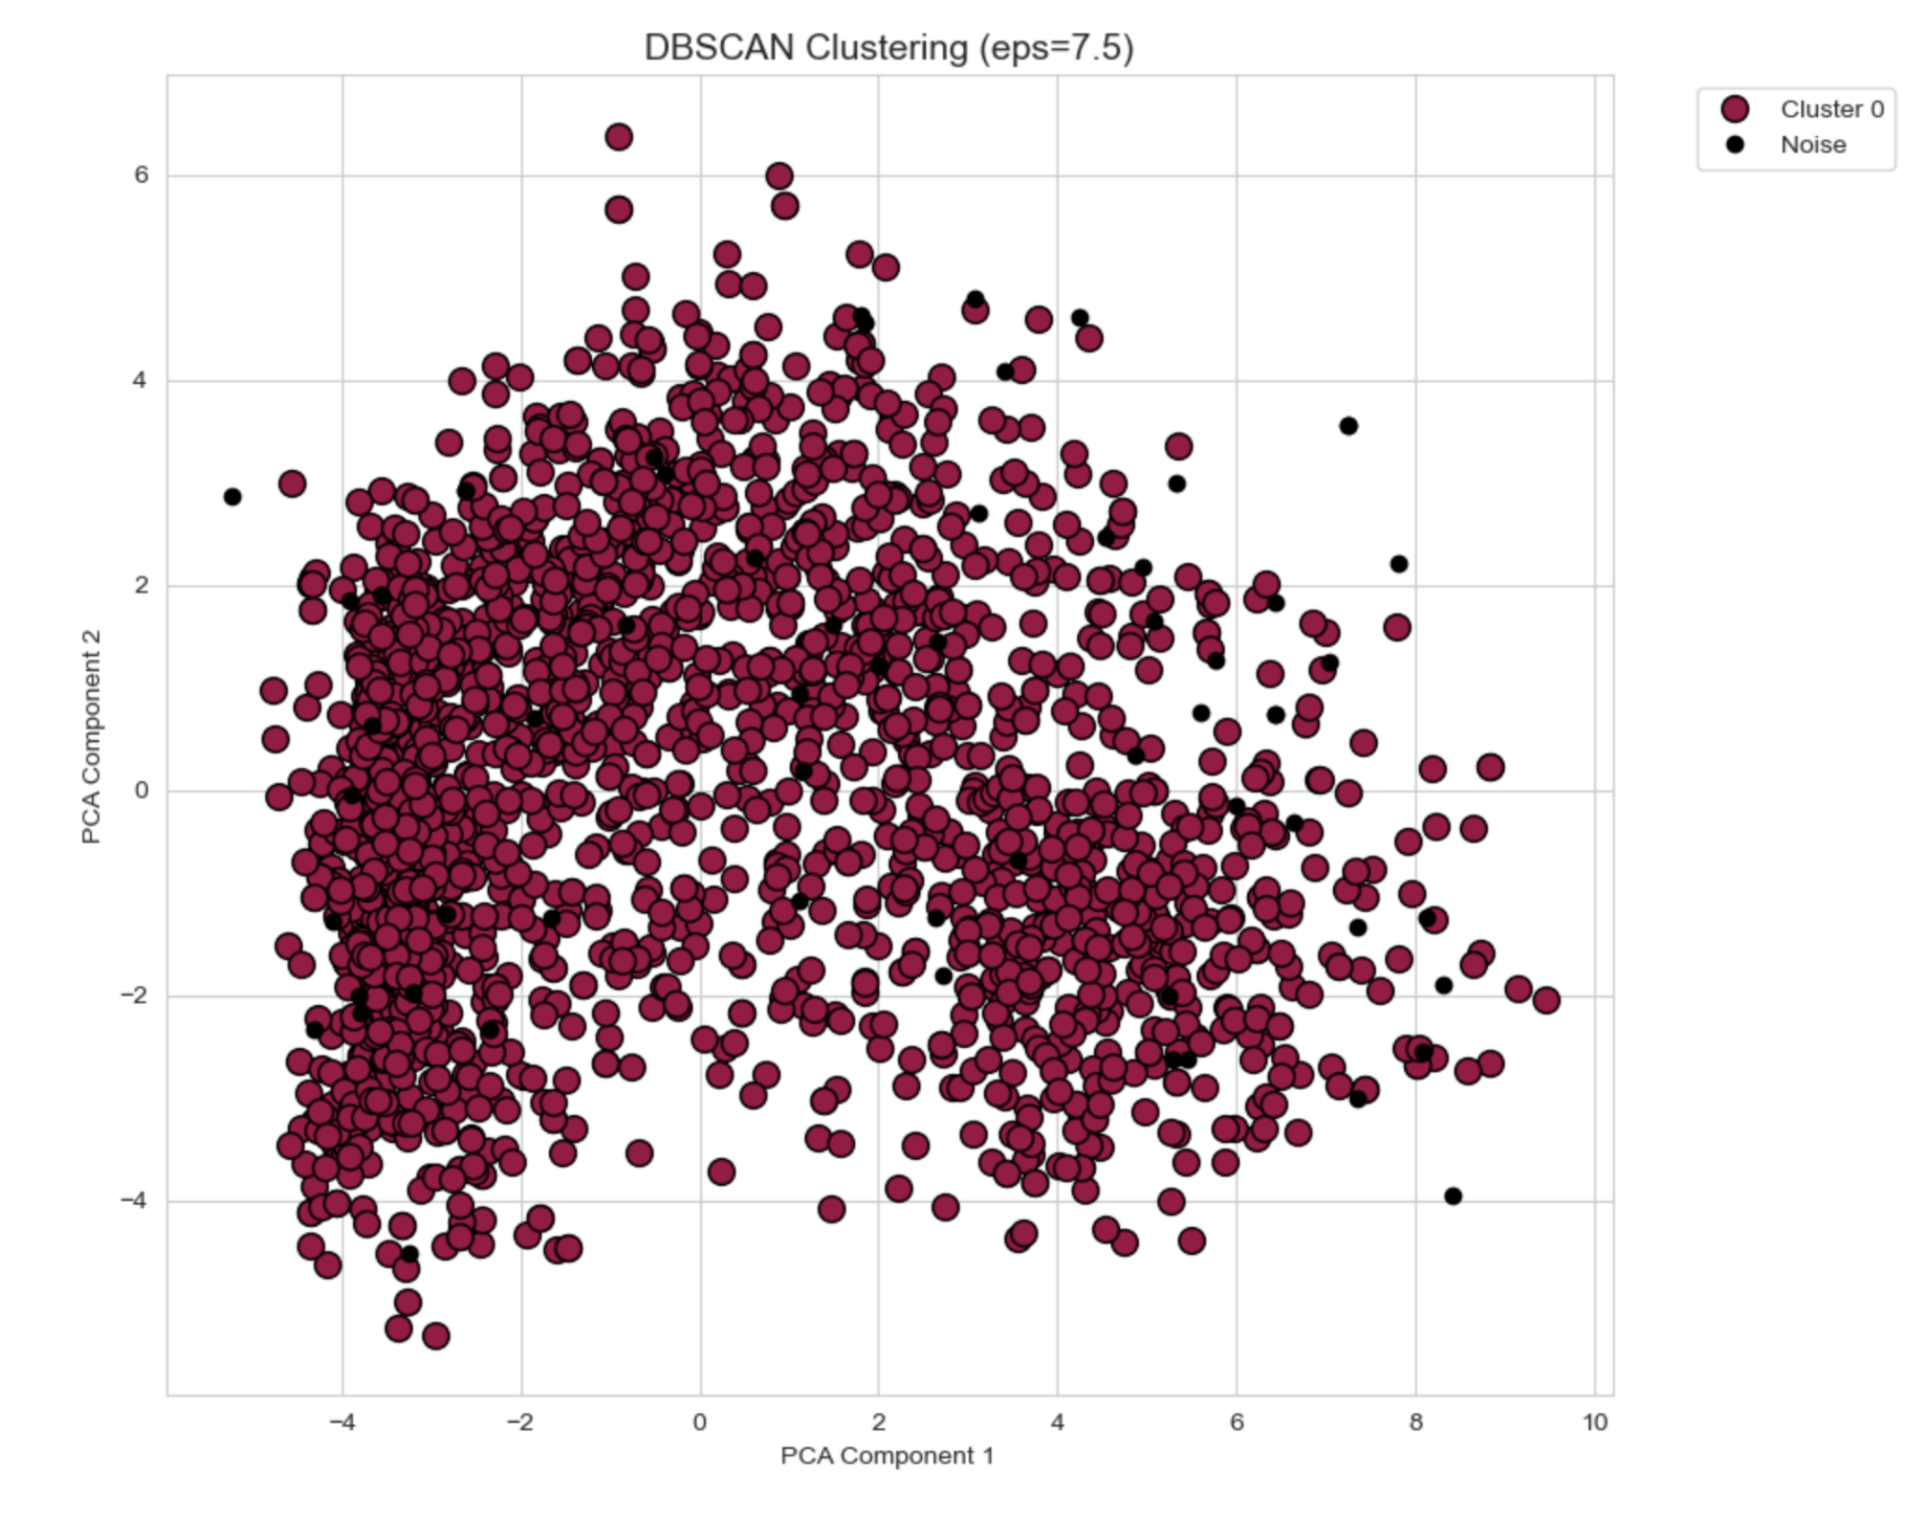
\includegraphics[width=0.8\textwidth]{DBSCAN.png}



\subsection{Campaign Response Prediction}

The dataset contains response to marketing campaign score, it measures the engagement of a consumer to a marketing campaign. Therefore, we fitted a Logistic Regression, a Random Forest and a XGBoost to try and predict the score of the marketing campaign response for an individual. Logistic Regression has shown to be the most effective method with a ROC of around 90\%, displaying a strong ability to classify the clients based on their probability of response. Furthermore, the model's precision was of 70\% indicating that 7 people labelled as responder out of ten would actually respond to the campaign. This allows for a far better ROI as opposed to generalised campaign cutting cost by 50\%. These results imply a better optimization of the budget coupled with a better customer experience since the clients would be less spammed with marketing campaigns. Finally this model affects the logistic aspect of the retail work as well. Indeed, it allows the forecast of campaign-driven demand, which allows the company to prepare sufficient stock in advance.

\begin{table}[H]
\centering
\caption{Model Performance Comparison for Campaign Response Prediction}
\begin{tabular}{lccccc}
\toprule
\textbf{Model} & \textbf{Accuracy} & \textbf{Precision} & \textbf{Recall} & \textbf{F1 Score} & \textbf{ROC AUC} \\
\midrule
Logistic Regression & 0.8931 & 0.7042 & 0.50 & 0.5848 & 0.9129 \\
Random Forest & 0.8705 & 0.5946 & 0.44 & 0.5057 & 0.8801 \\
Gradient Boosting & 0.8886 & 0.6757 & 0.50 & 0.5747 & 0.9005 \\
\midrule
\textbf{Best model:} & \multicolumn{5}{l}{\textbf{Logistic Regression}} \\
\bottomrule
\end{tabular}
\label{tab:campaign_results}
\end{table}

\subsection{Churn Prediction}

A customer churns when he becomes inactive and thus does not appear to buy the products of the retail company anymore. We therefore defined clients that churned as clients who did not make any orders 45 days after their last purchase. We then fitted a Logistic Regression, a Random Forest and a XGBoost to try and predict whether a customer had churned. Unlike for the precedent predictive task, the best performing model was the XGBoost. Its accuracy was moderate (around 60\%). It had a balanced recall (68\%) and precision (61\%), flagging correctly the customer at risk of churning 61\% of the time and identifying 68\% of the time the clients that actually churned. Its ROC was 64\% displaying a meaningful discriminative ability. Hence the flagged 20\% most likely to churn have a genuine higher risk to do so. This model can allow for a proactive retention campaign focussed on the 25\% of the clients who have the highest expected churn rate (between 80 and 90\%). Such campaigns could include discounts, free shipping or bonus loyalty points.



\includegraphics[width=0.8\textwidth]{churn.png} 


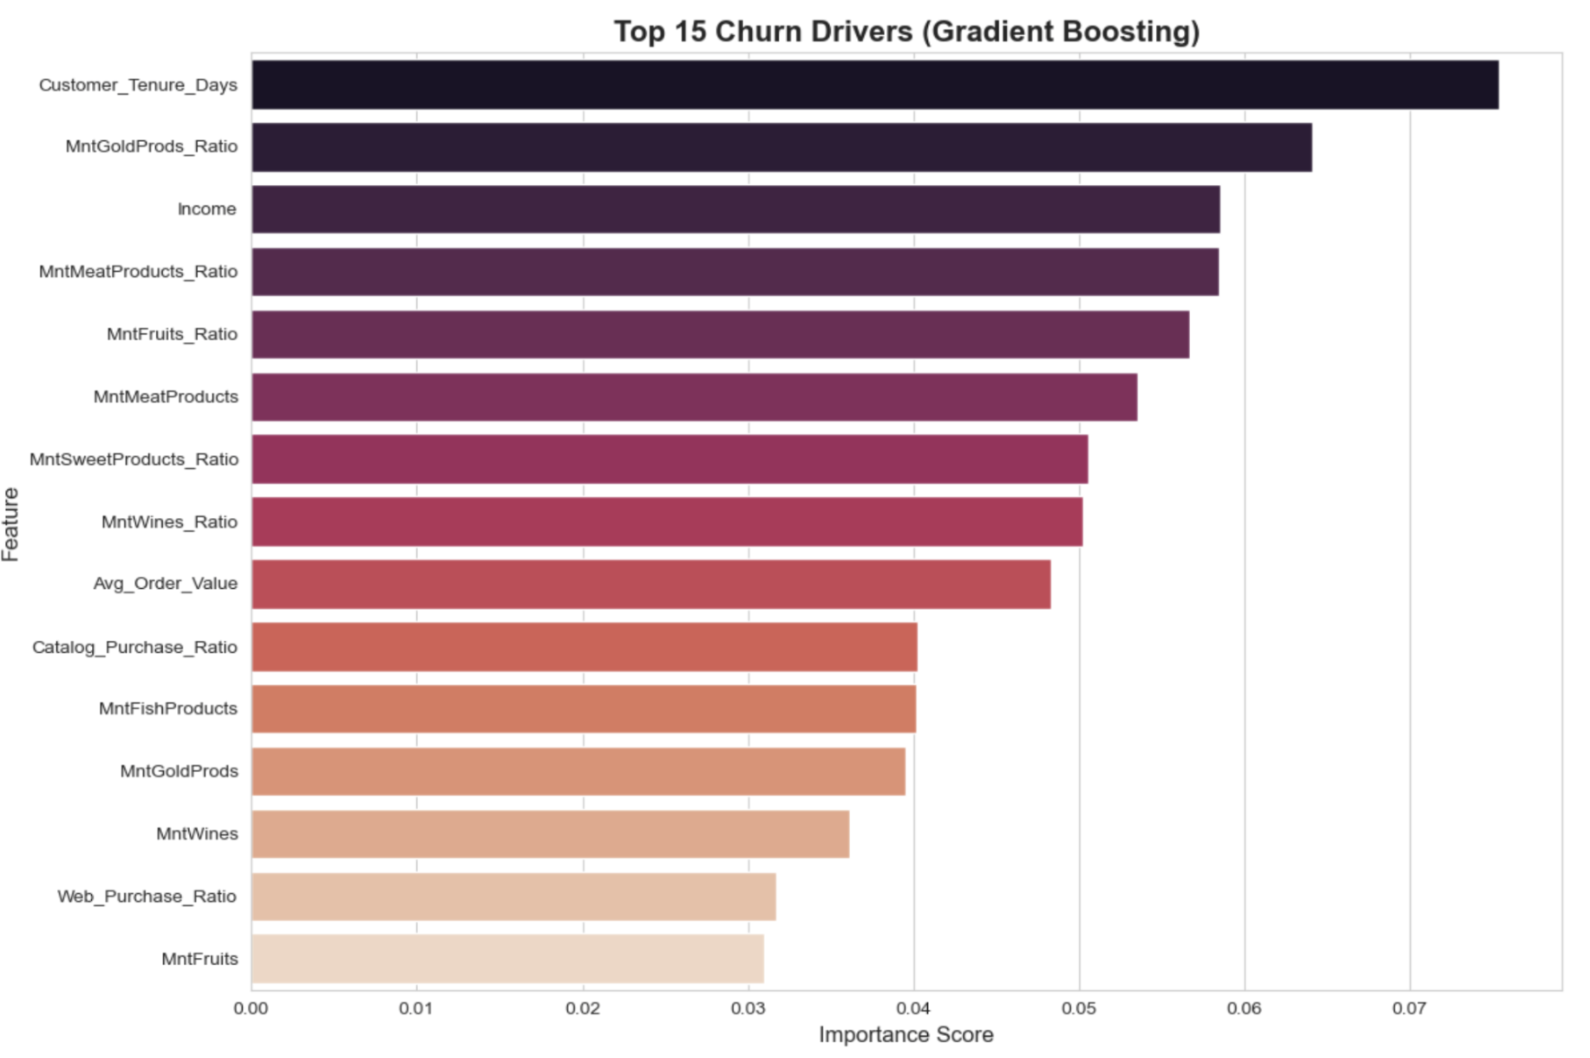
\includegraphics[width=0.95\textwidth]{drivers.png}


\section{Conclusion}

This research demonstrates how machine learning techniques can support retailers in improving marketing operations and customer loyalty initiatives through data-driven analysis. The homogeneous structure of the dataset limited the effectiveness of clustering algorithms in identifying meaningful customer segments; however, supervised learning models delivered actionable results. Logistic regression achieved the strongest performance in campaign response prediction, enabling more effective and targeted marketing strategies. XGBoost produced moderate but useful results for churn prediction, allowing retailers to identify high-risk customers and initiate early retention actions. Overall, these models provide a practical approach to increasing marketing return on investment and customer lifetime value, while future improvements could be achieved through richer data and enhanced feature engineering.

\bibliographystyle{apalike}
\begin{thebibliography}{9}

\bibitem{reichheld1990}
Reichheld, Frederick F., and W. Earl Sasser, Jr.
\textit{Zero Defections: Quality Comes to Services.}
Harvard Business Review, vol. 68, no. 5, 1990, pp. 105--11.

\bibitem{imakash3011}
Imakash3011. (n.d.).
\textit{Customer Personality Analysis [Data set].}
Kaggle.
\url{https://www.kaggle.com/datasets/imakash3011/customer-personality-analysis}

\bibitem{github}
Das M, de Leusse A, Vannson A. (n.d.).
\textit{DataForge-Labs (Version main) [Analysis repository].}
Retrieved from \url{https://github.com/alexisvannson/DataForge-Labs/tree/main}

\end{thebibliography}

\end{document}